\chapter{Design}

\section{Overall System Design}

\begin{itemize}
	\item
	\item
\end{itemize}

\subsection{Short description of the main parts of the system}

\subsection{System flowcharts showing an overview of the complete system}

Key:
\begin{figure}[H]
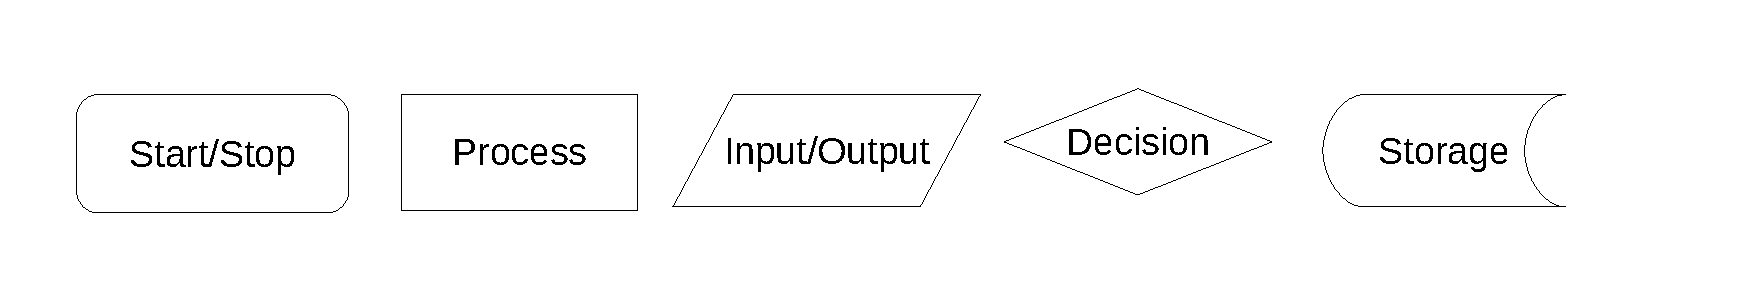
\includegraphics[width=\textwidth]{./Design/images/FC_key.pdf}
    \caption{Key for flow chart} \label{fig:Flow Chart Key}
\end{figure}

Start of the flow chart:
\begin{figure}[H]
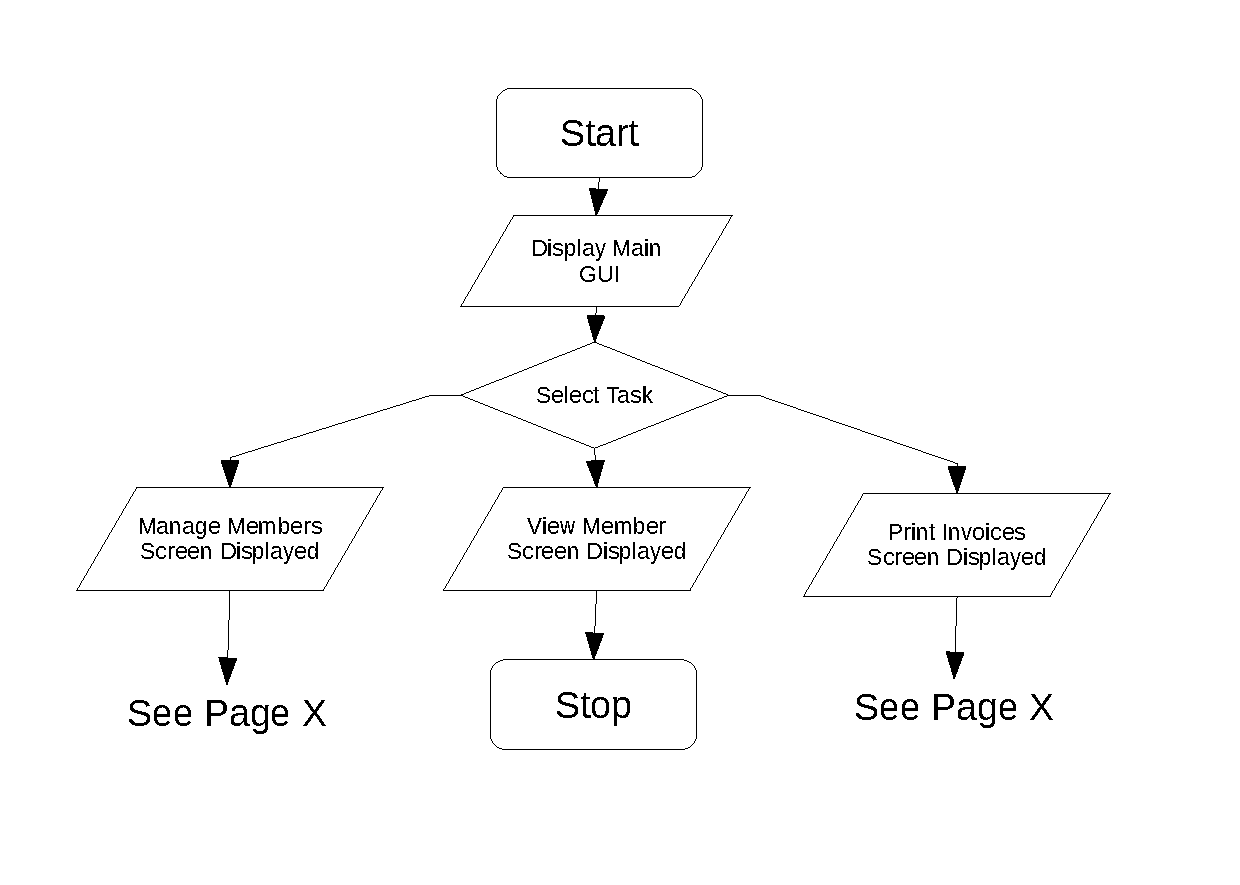
\includegraphics[width=\textwidth]{./Design/images/FC_start.pdf}
    \caption{Start of flow chart} \label{fig:Flow Chart Start}
\end{figure}

Managing members:
\begin{figure}[H]
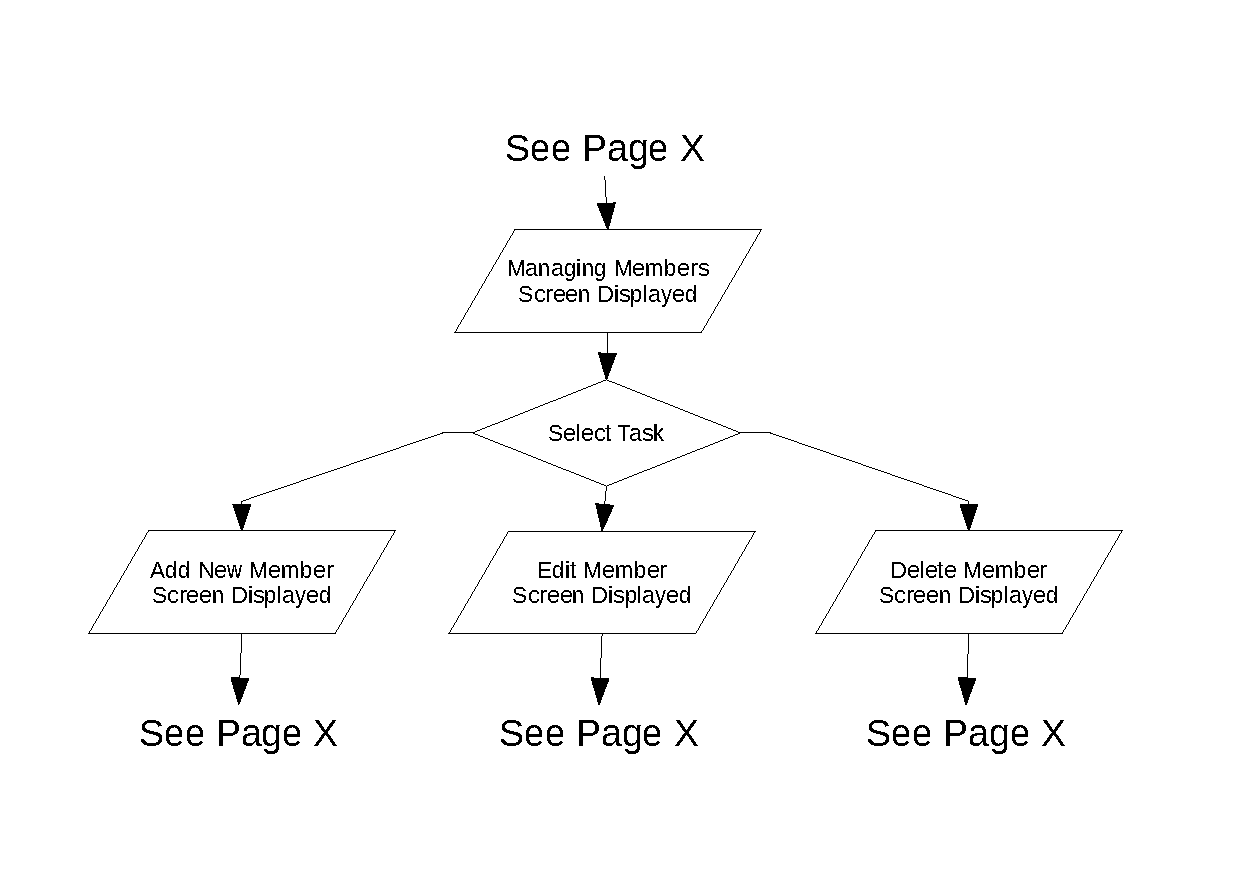
\includegraphics[width=\textwidth]{./Design/images/FC_manage_members.pdf}
    \caption{Manage Members} \label{fig:Flow Chart Manage Members}
\end{figure}

Editing a member:
\begin{figure}[H]
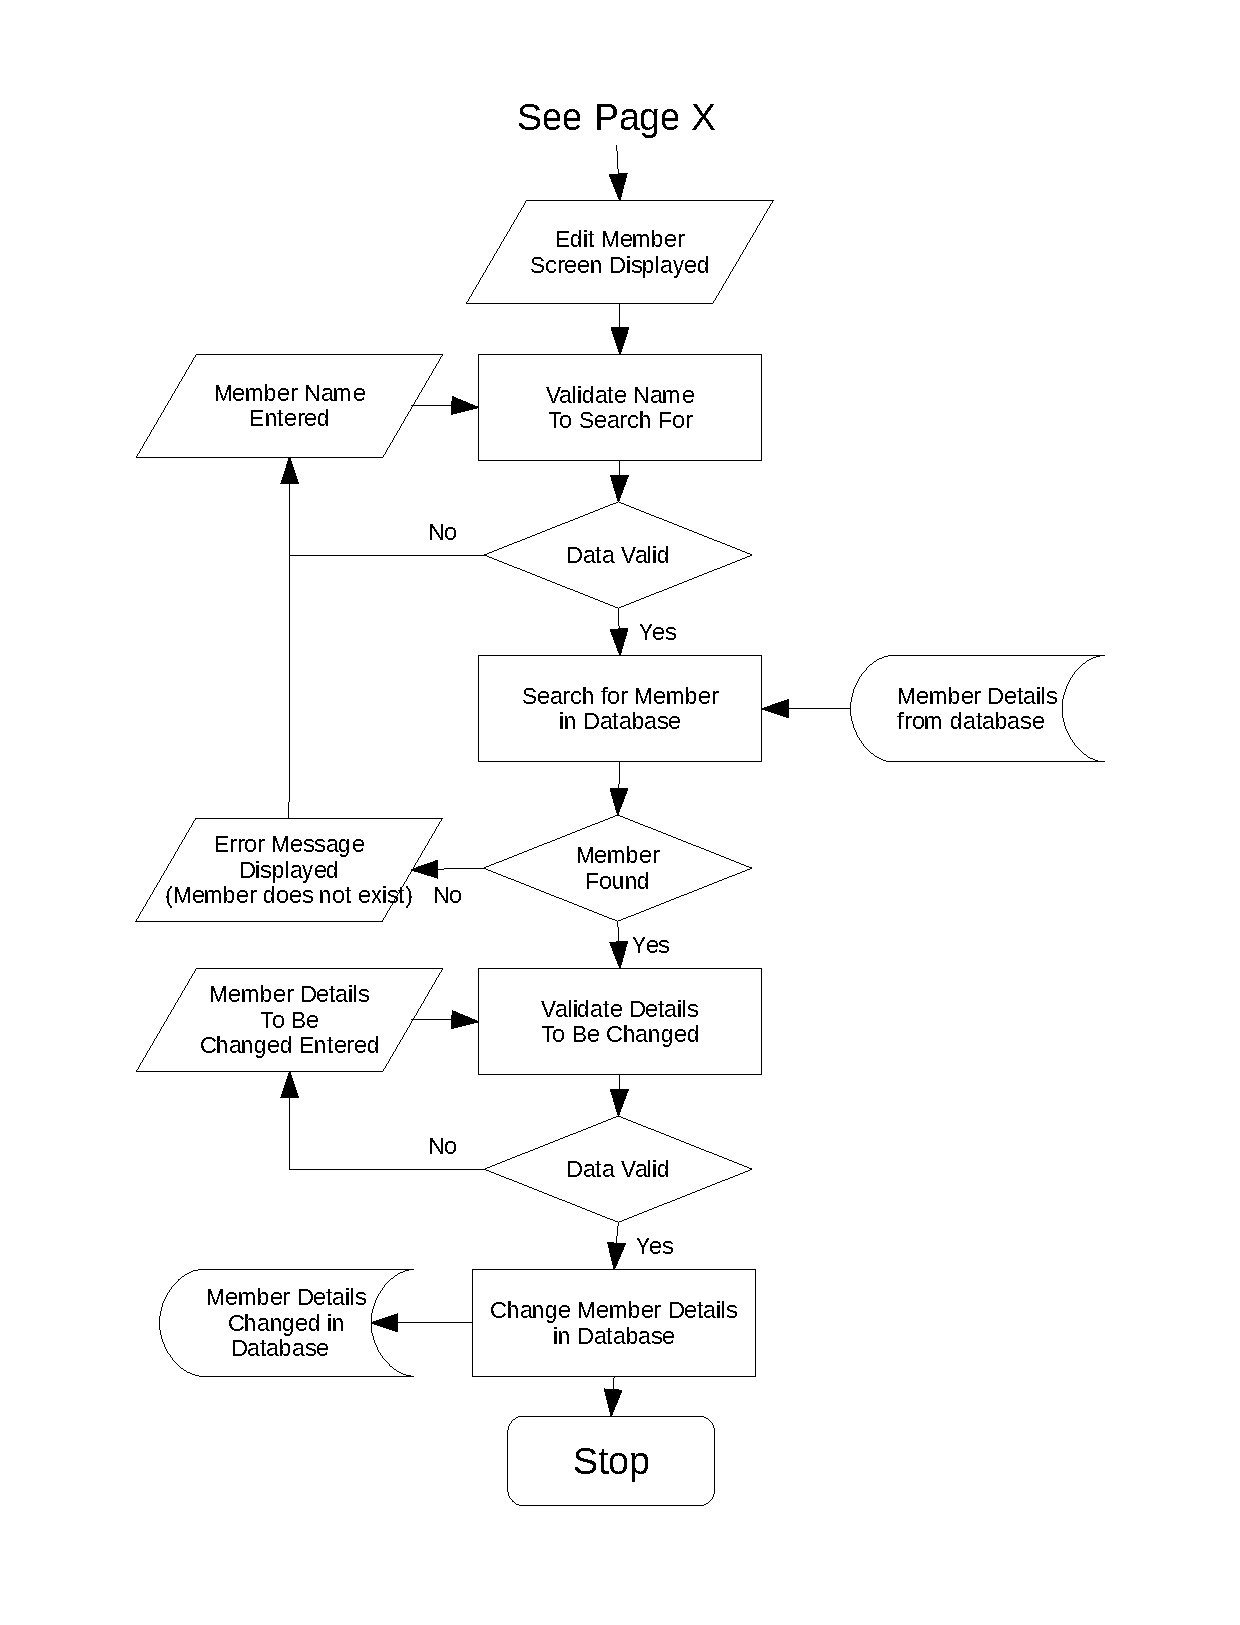
\includegraphics[width=\textwidth]{./Design/images/FC_edit_member.pdf}
    \caption{Edit Member} \label{fig:Flow Chart Edit Member}
\end{figure}

Deleting a member:
\begin{figure}[H]
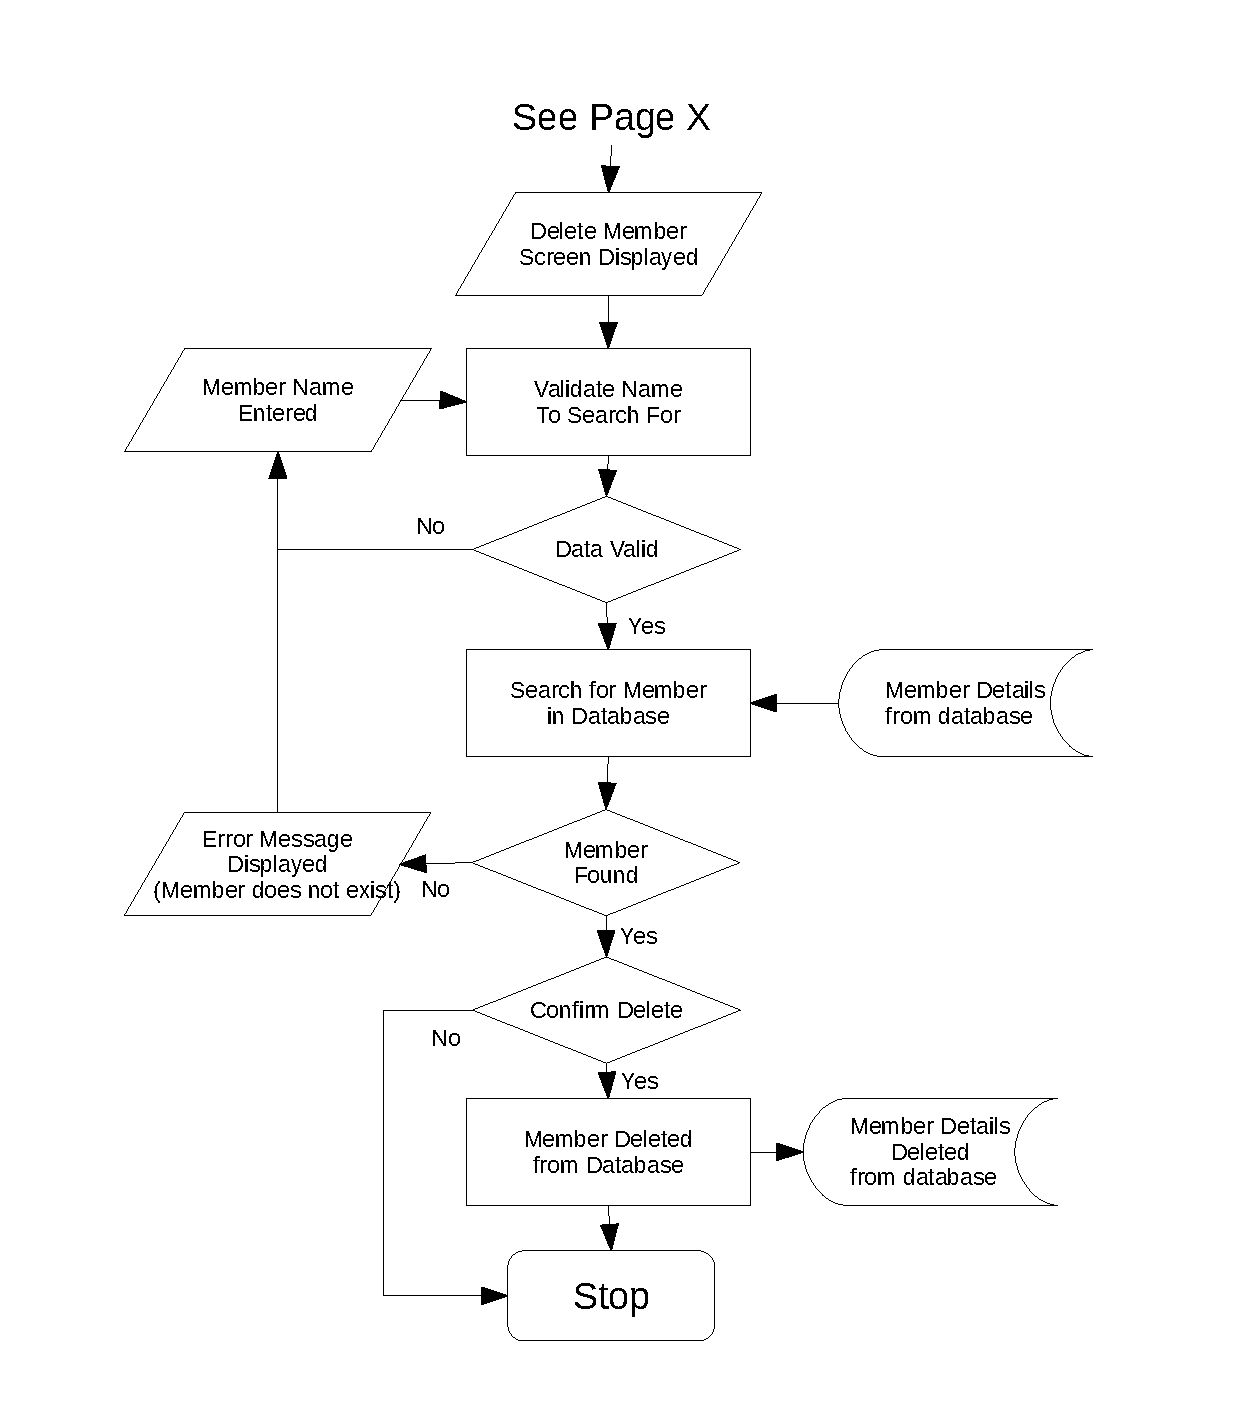
\includegraphics[width=\textwidth]{./Design/images/FC_delete_member.pdf}
    \caption{Delete Member} \label{fig:Flow Chart Delete Member}
\end{figure}

Adding a new member:
\begin{figure}[H]
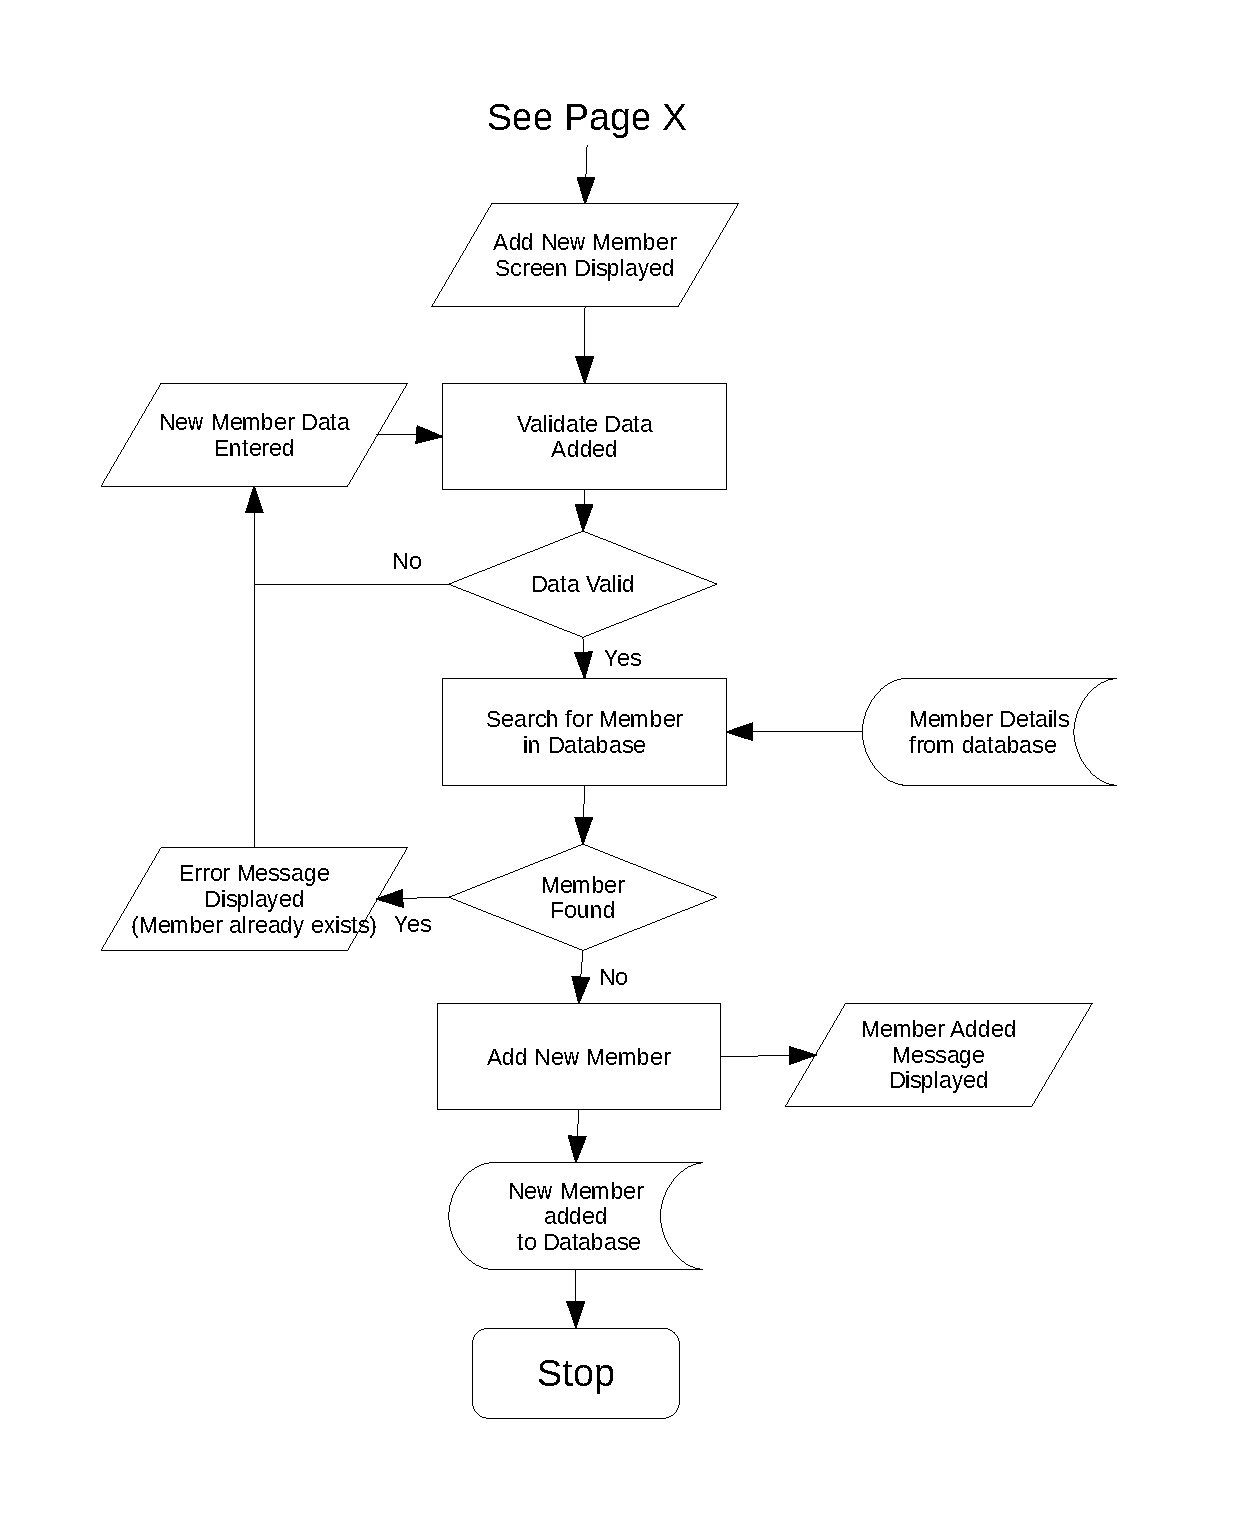
\includegraphics[width=\textwidth]{./Design/images/FC_add_new_member.pdf}
    \caption{Add New Member} \label{fig:Flow Chart Add New Member}
\end{figure}

Printing the invoices:
\begin{figure}[H]
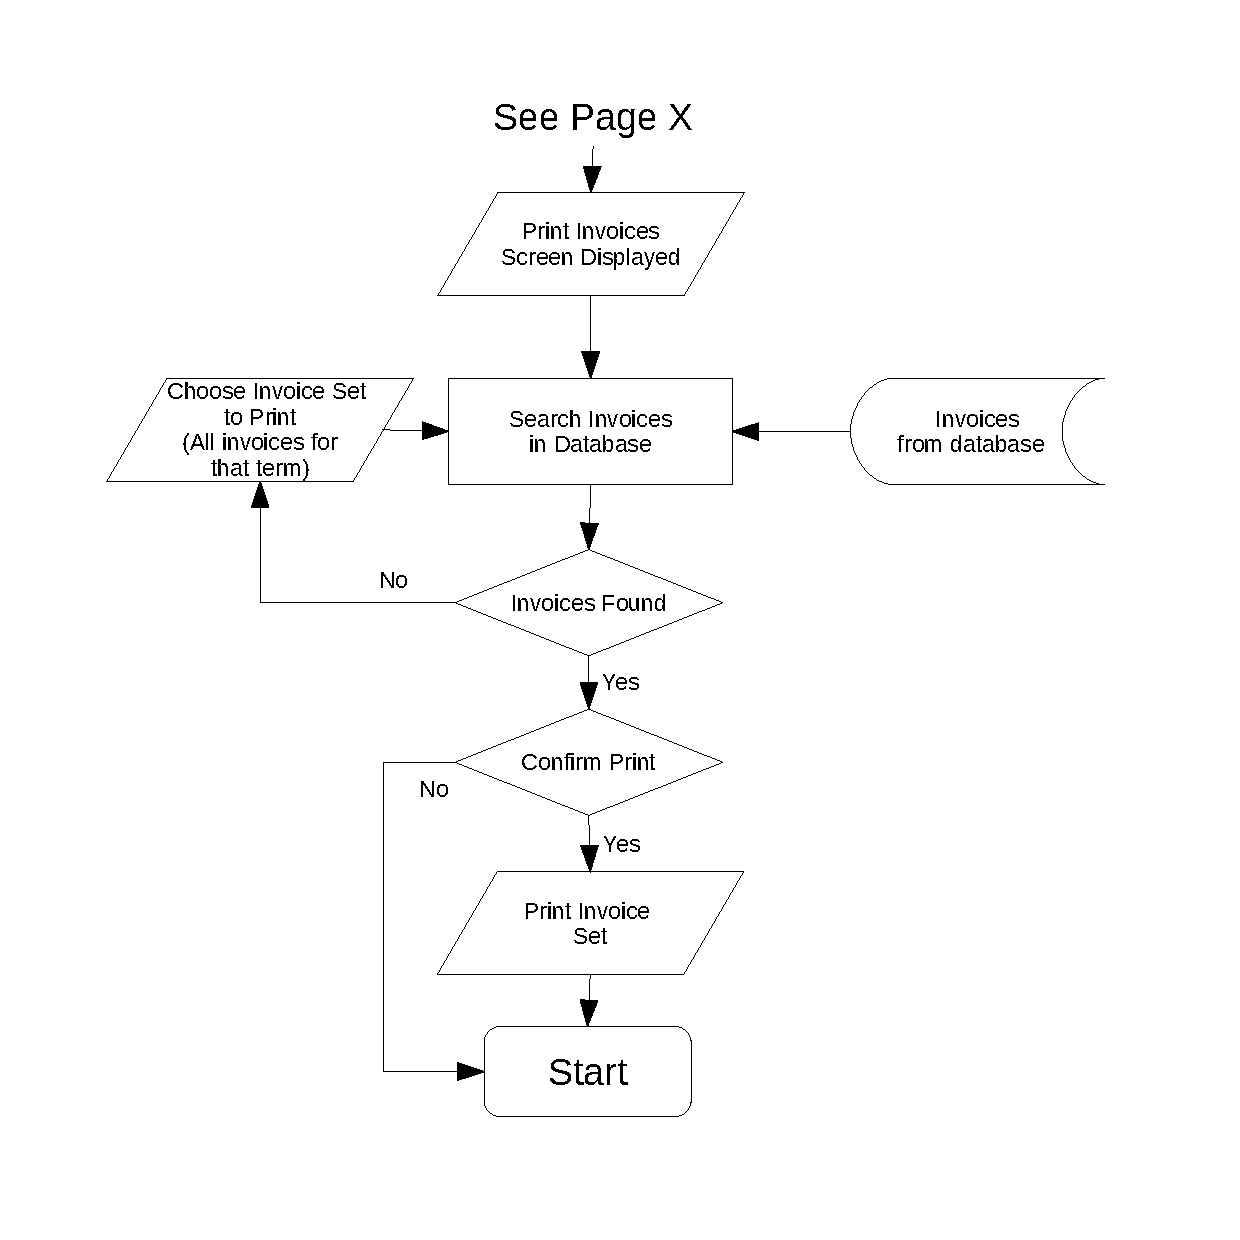
\includegraphics[width=\textwidth]{./Design/images/FC_print_invoices.pdf}
    \caption{Print Invoices} \label{fig:Flow Chart Print Invoices}
\end{figure}

\section{User Interface Designs}

\section{Hardware Specification}
No extra hardware will be needed.

\section{Program Structure}

\subsection{Top-down design structure charts}

\subsection{Algorithms in pseudo-code for each data transformation process}

\begin{algorithm}[H]
\label{fig:repeat_pseudo_example}
    \caption{Repeat Loop}
\begin{algorithmic}[1]
\SET{$total$}{$0$}
\State
\Repeat
    \SEND{$"Please\ enter\ a\ number\ (0 to finish)"$}
    \RECEIVE{$number$}
    \SET{$total$}{$total + number$}
\Until{$number = 0$}
\end{algorithmic}
\end{algorithm}

\subsection{Object Diagrams}

\subsection{Class Definitions}

\section{Prototyping}

\section{Definition of Data Requirements}

\subsection{Identification of all data input items}

\subsection{Identification of all data output items}

\subsection{Explanation of how data output items are generated}

\subsection{Data Dictionary}

\newpage
\begin{center}
\begin{tabular}{|p{2cm}|p{2cm}|p{2cm}|p{2cm}|l}
\hline
\textbf{Name}                    & \textbf{Data Type}    & \textbf{Length}                  & \textbf{Validation} \\ \hline
MemberID                           & String            & 4 digits                & Numbers only \\ \hline
ParentID                             & String            & 4 digits                & Numbers only \\ \hline
Member first name              & String            & 1-20 characters   & Letters only \\ \hline
Member last name               & String           &1-20 characters &  Letters only \\ \hline
Parents first name               & String           & 1-20 characters &  Letters only \\ \hline
Parent last name                 & String           & 1-20 characters &  Letters only \\ \hline
Member town name                 & String           & 1-20 characters &  Letters only \\ \hline
Member street name                 & String           & 1-20 characters &  Letters only \\ \hline
Member house name/number & String              & 1-20 characters &  Letters only \\ \hline
Parent town name                 & String           & 1-20 characters &  Letters only \\ \hline
Parent street name                 & String           & 1-20 characters &  Letters only \\ \hline
Parent house name/number & String                 & 1-20 characters &  Letters only \\ \hline
Parent primary phone number         & Integer        & 12 digits & Numbers only, correct format and a valid phone number \\ \hline
Parent secondary phone number         & Integer        & 12 digits & Numbers only, correct format and a valid phone number \\ \hline
Parent email                        & String          & 1-30 characters &  Letters only \\ \hline
Member date of birth          & Datetime       & 6 digits & Numbers only (dd/mm/yy) \\ \hline
Invoice ID                           & Integer       & 4 digits & Numbers only \\ \hline
Was invoice paid                 & Integer       & 4-6 digits & Numbers only, correct format and a valid date \\ \hline
Date invoice was sent        & Datetime       & 6 digits & Numbers only (dd/mm/yy) \\ \hline
\end{tabular}
\end{center}

\subsection{Identification of appropriate storage media}

\section{Database Design}

\subsection{Normalisation}

\subsubsection{ER Diagrams}

ER diagram of the fully normalised database:
\begin{figure}[H]
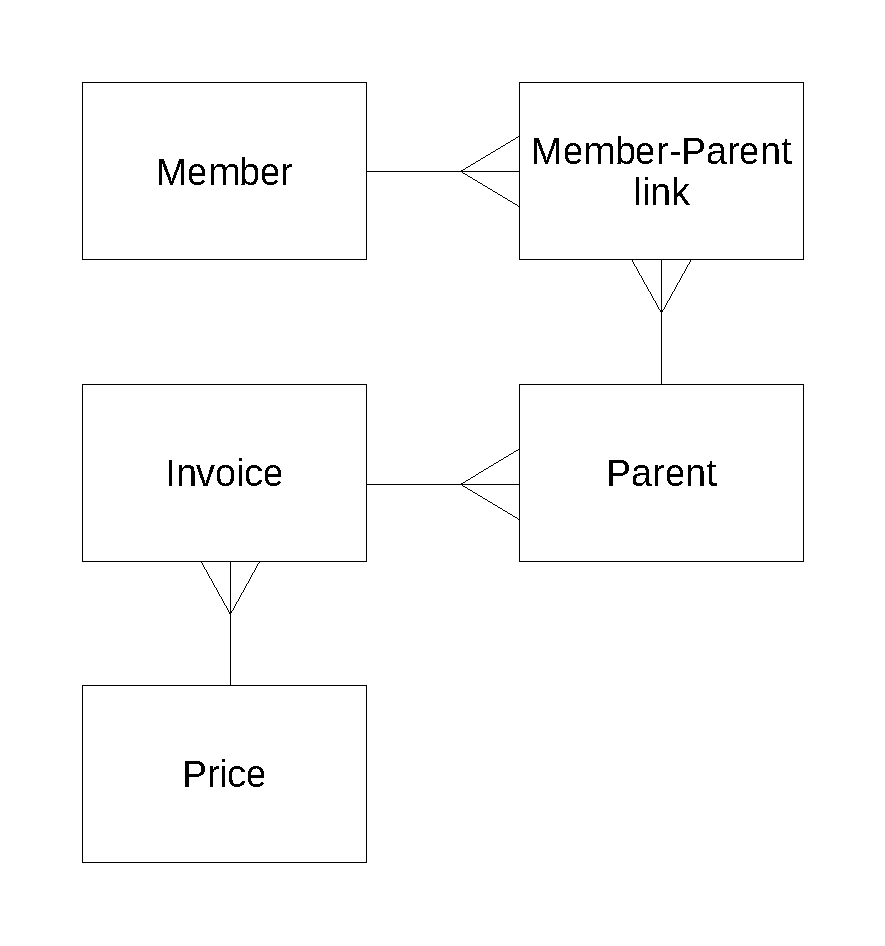
\includegraphics[width=\textwidth]{./Design/images/ER_diagram_design.pdf}
    \caption{ER diagram of the fully normalised database} \label{fig:ER_diagram_design}
\end{figure}


\subsubsection{Entity Descriptions}

\subsubsection{1NF to 3NF}

\begin{figure}[H]
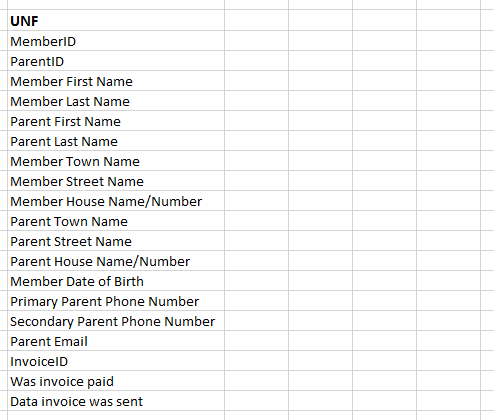
\includegraphics[width=\textwidth]{./Design/images/UNF.png}
    \caption{UNF of database} \label{fig:UNF}
\end{figure}

\begin{center}
	\begin{tabular}{|p{4cm}|p{4cm}|}
		\hline
		MemberID
		ParentID
		Member First Name
		Member Last Name
		Parent First Name
		Parent Last Name
		Member Town Name
		Member Street Name
		Member House Name/Number
		Parent Town Name
		Parent Street Name
		Parent House Name/Number
		Member Date of Birth
		Primary Parent Phone Number
		Secondary Parent Phone Number
		Parent Email
		InvoiceID
		Was invoice paid
		Data invoice was sent
		PriceID
		Term Price
		Sibling discount amount
	\end{tabular}
\end{center}


1. Split the attributes into repeating and non-repeating groups. Create a composite key in the repeating group.

\begin{figure}[H]
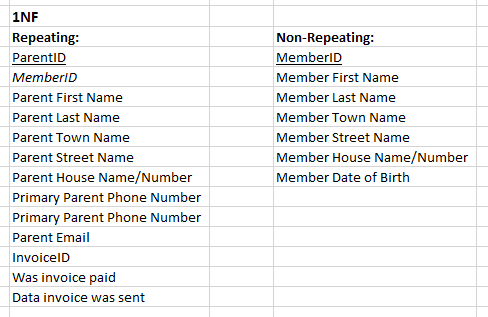
\includegraphics[width=\textwidth]{./Design/images/1NF.png}
    \caption{1NF of database} \label{fig:UNF}
\end{figure}

2. Remove any attributes that do not rely on both parts of the composite key from the repeating group and add the key they do rely on to the new group.

\begin{figure}[H]
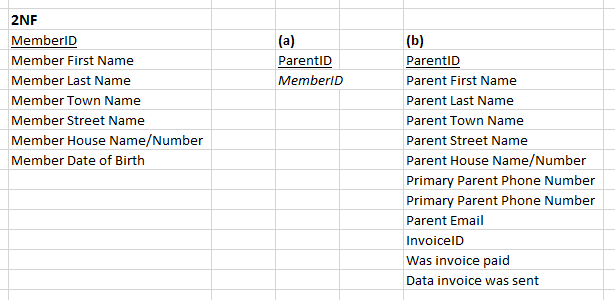
\includegraphics[width=\textwidth]{./Design/images/2NF.png}
    \caption{2NF of database} \label{fig:UNF}
\end{figure}

3. Split the new group further so all attributes are in a group with a primary key they directly relate to.

\begin{figure}[H]
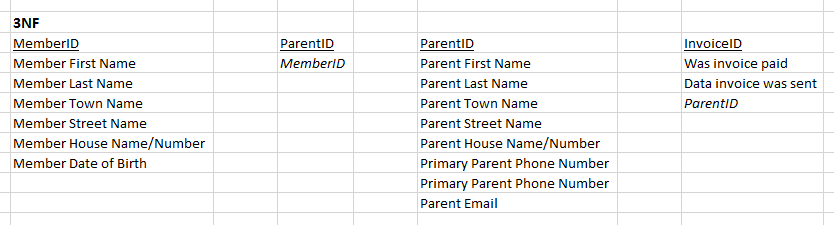
\includegraphics[width=\textwidth]{./Design/images/3NF.png}
    \caption{3NF of database} \label{fig:UNF}
\end{figure}

Member\textbf{(MemberID},Member First Name, Member Last Name, Member Town Name, Member Street Name, Member house Name/Number, Member Date of Birth)

Parent-Member({\textbf{ParentID},\textit{MemberID})

Parent(\textbf{ParentID}, Parent First Name, Parent Last Name, Parent Town Name, Parent Street Name, Parent house Name/Number,  Parent Email, Parent Phone Number)

Invoice(\textbf{InvoiceID}, \textit{ParentID}, \textit{PriceID}, Was Invoice Paid, Date Invoice Was Sent)

Price(\textbf{PriceID}, Term Price, Sibling Discount)

\section{Security and Integrity of the System and Data}

\subsection{Security and Integrity of Data}

\subsection{System Security}

\section{Validation}

\section{Testing}

\begin{landscape}
\subsection{Outline Plan}

\begin{center}
    \begin{tabular}{|p{2cm}|p{5cm}|p{5cm}|p{4cm}|}
        \hline
        \textbf{Test Series} & \textbf{Purpose of Test Series} & \textbf{Testing Strategy} & \textbf{Strategy Rationale}\\ \hline
        Example & Example & Example & Example \\ \hline
    \end{tabular}
\end{center}

\subsection{Detailed Plan}

\begin{center}
    \begin{longtable}{|p{1.5cm}|p{2.5cm}|p{2.5cm}|p{2cm}|p{2cm}|p{2cm}|p{2cm}|p{2cm}|}
        \hline
        \textbf{Test Series} & \textbf{Purpose of Test} & \textbf{Test Description} & \textbf{Test Data} & \textbf{Test Data Type (Normal/ Erroneous/ Boundary)} & \textbf{Expected Result} & \textbf{Actual Result} & \textbf{Evidence}\\ \hline
        Example & Example & Example & Example & Example & Example & Example & Example \\ \hline
    \end{longtable}
\end{center}
\end{landscape}
